\chapter{Evalución Continua 2}
\newpage
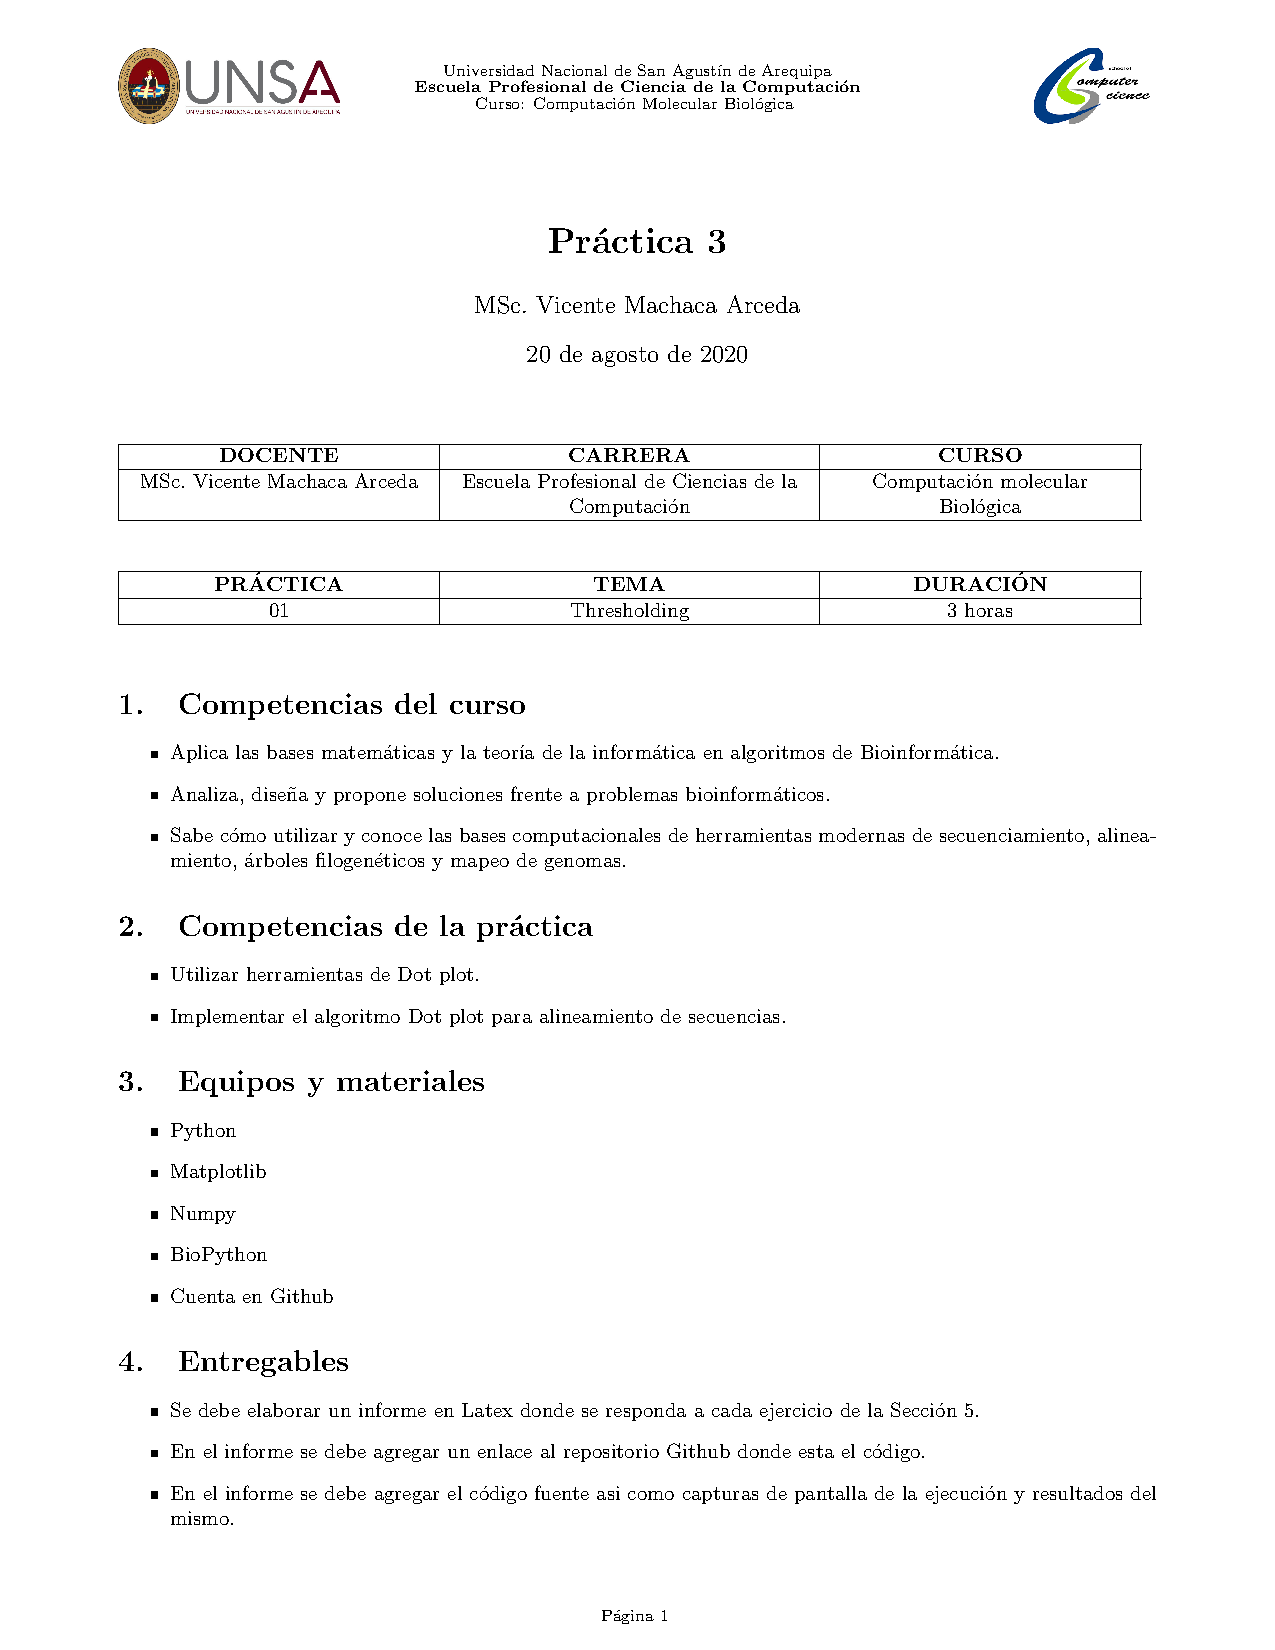
\includepdf[pages={1-}]{pdfs/practices/3_dot_matrix.pdf}
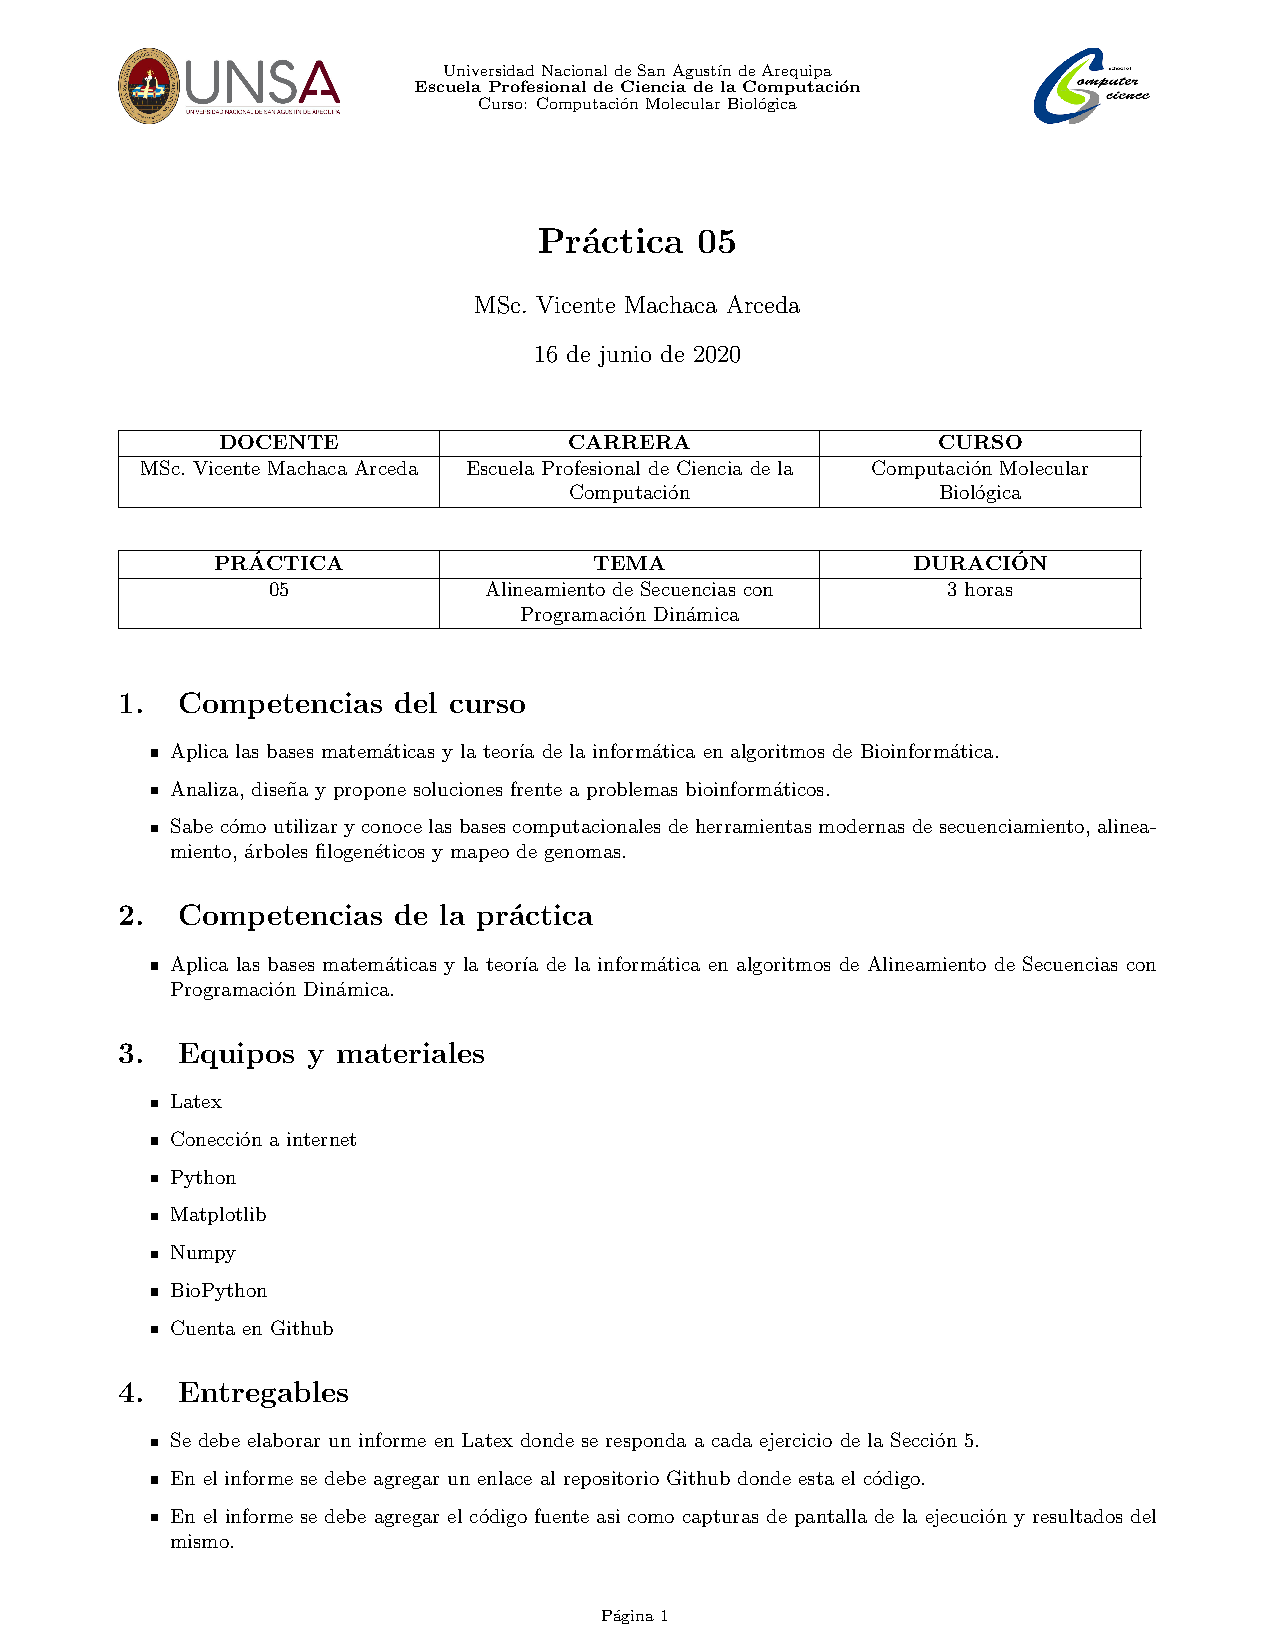
\includepdf[pages={1-}]{pdfs/practices/4_alignment.pdf}
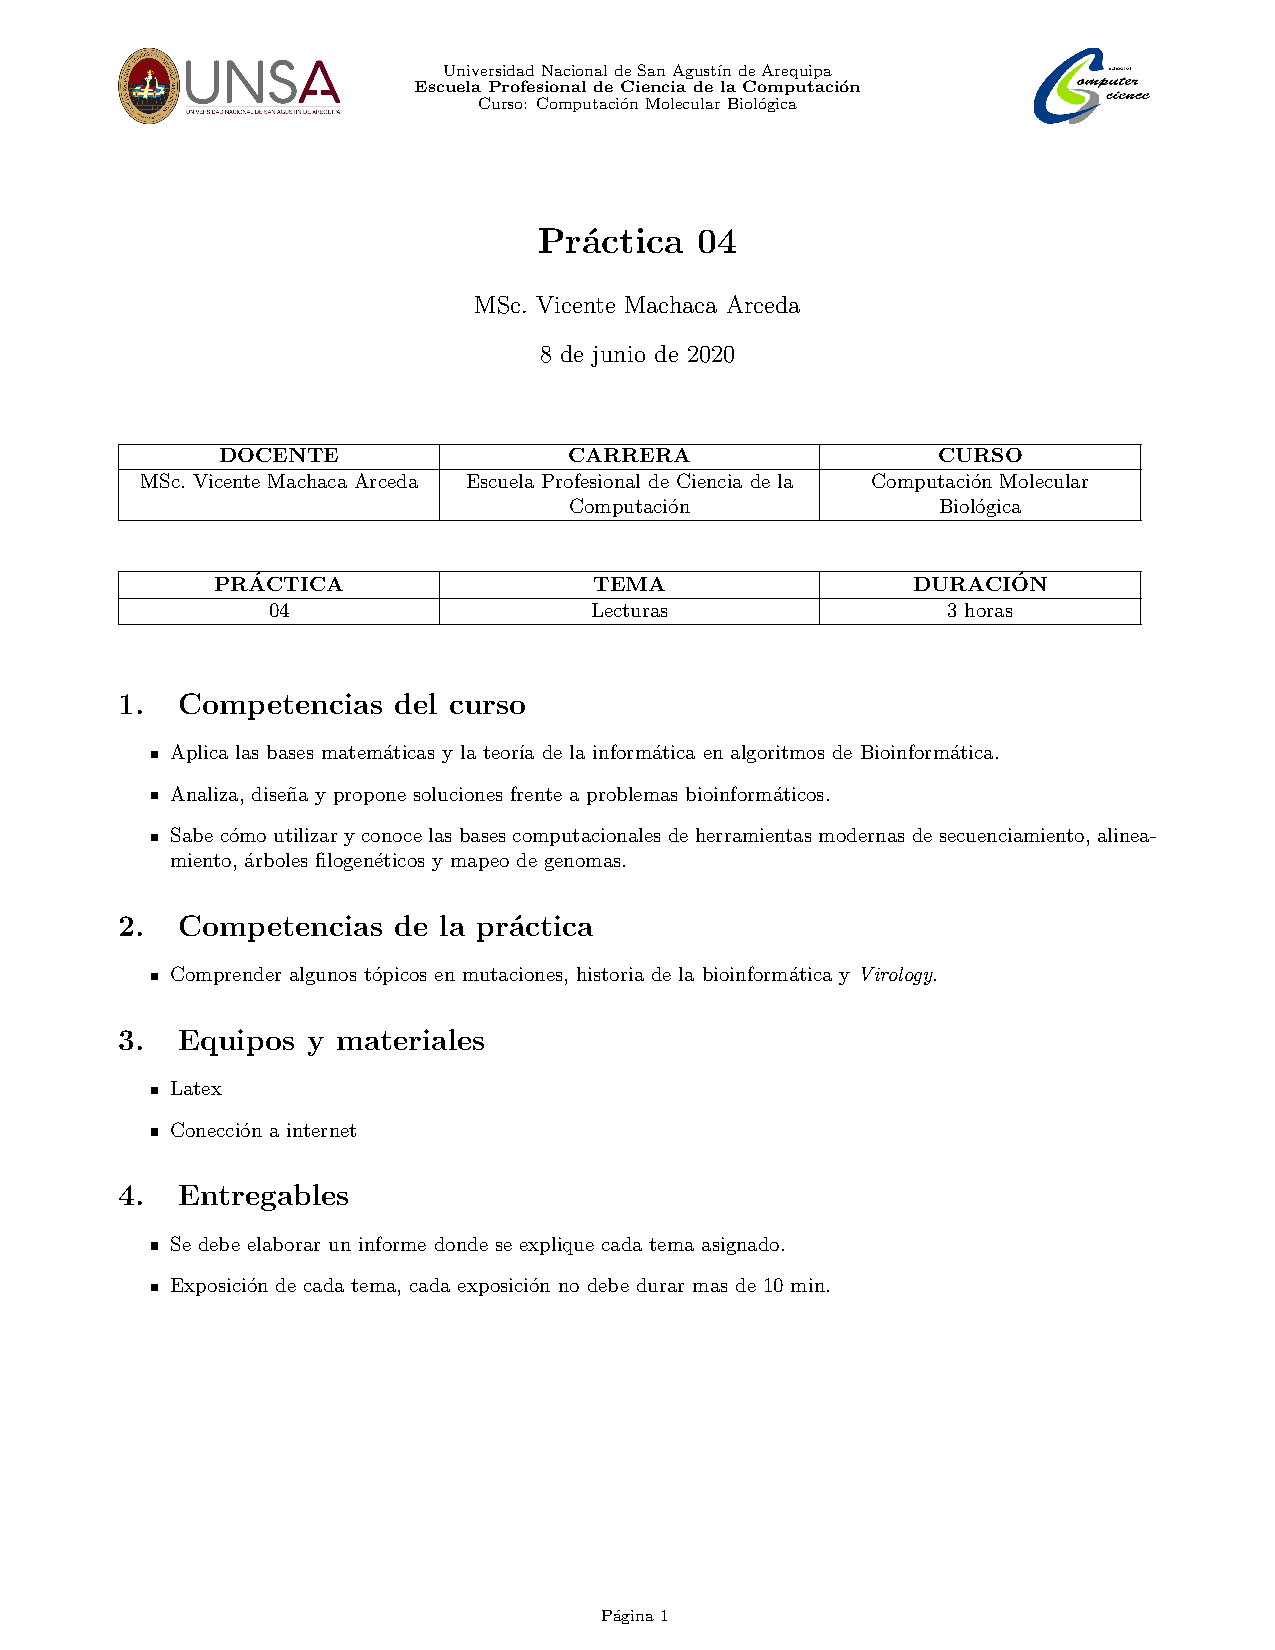
\includepdf[pages={1-}]{pdfs/practices/4_lectures.pdf}
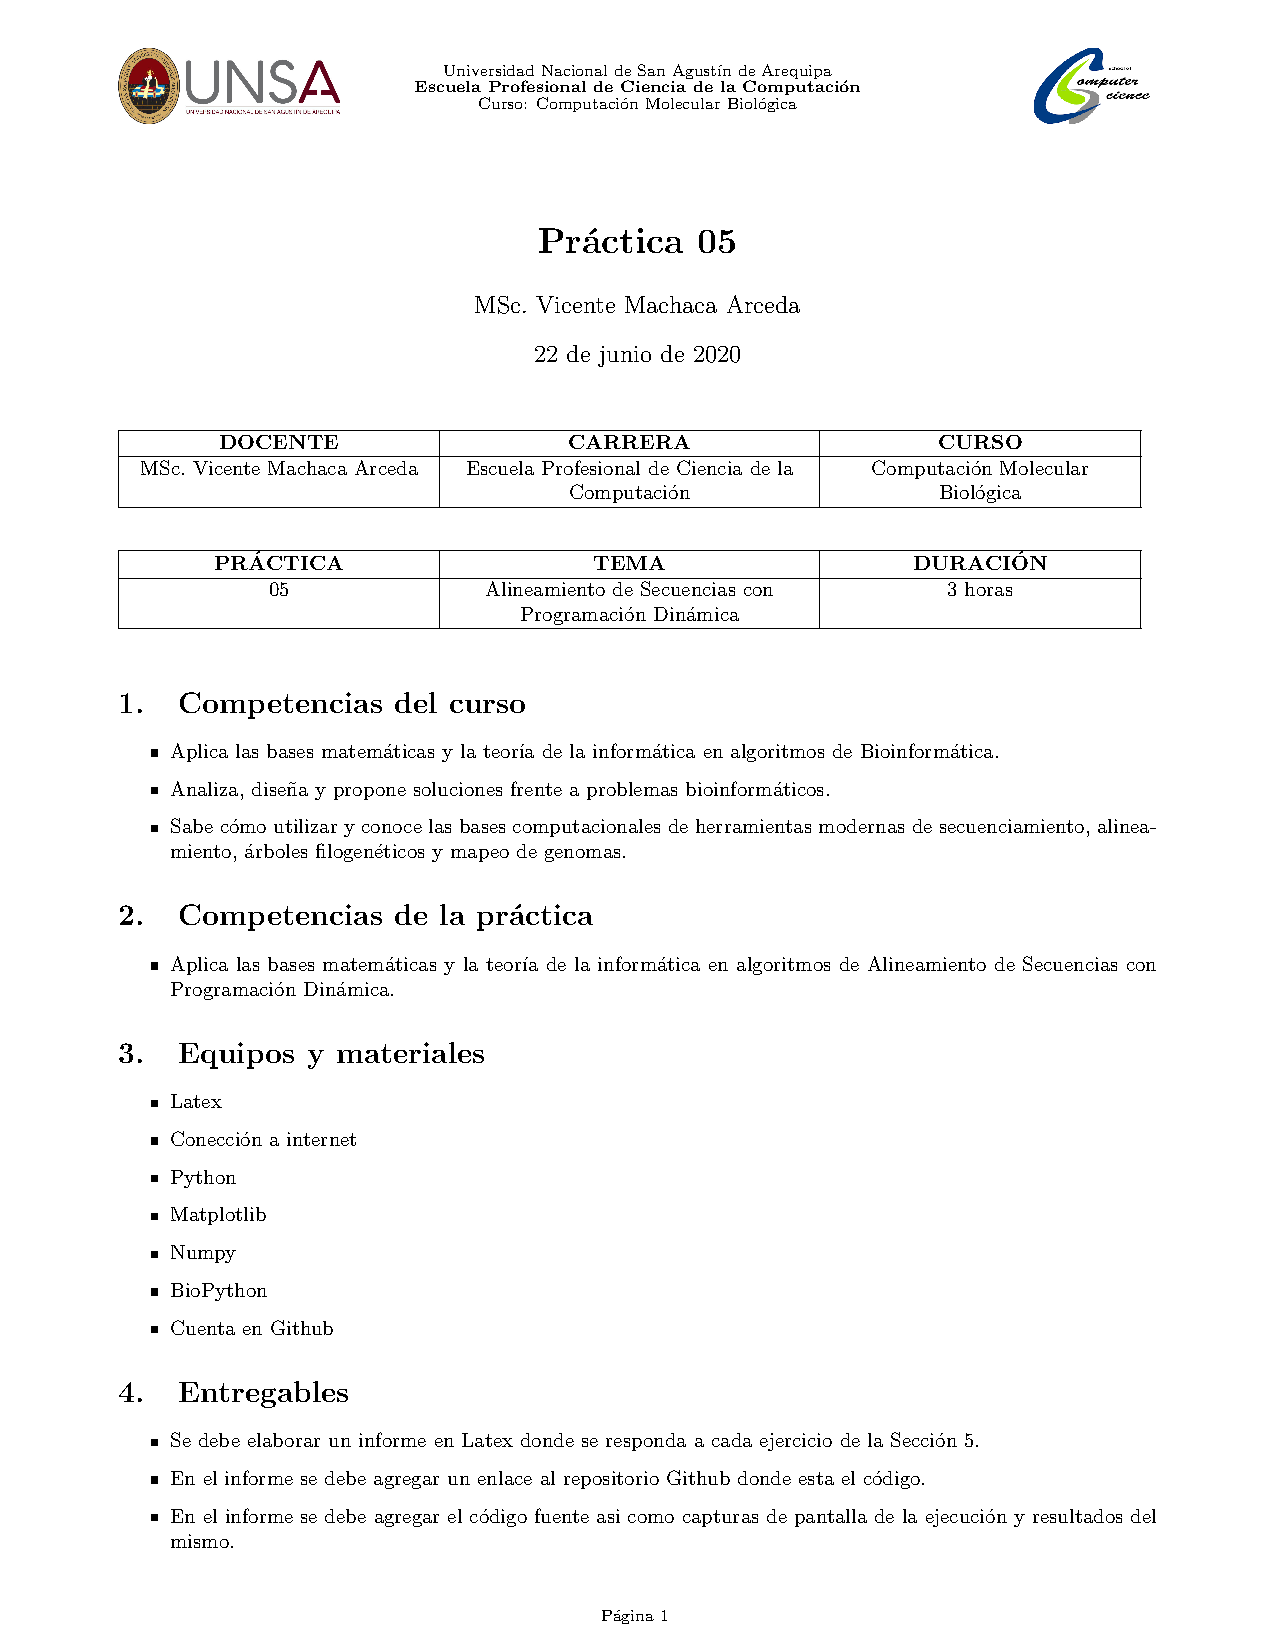
\includepdf[pages={1-}]{pdfs/practices/5_alignment_exercises.pdf}
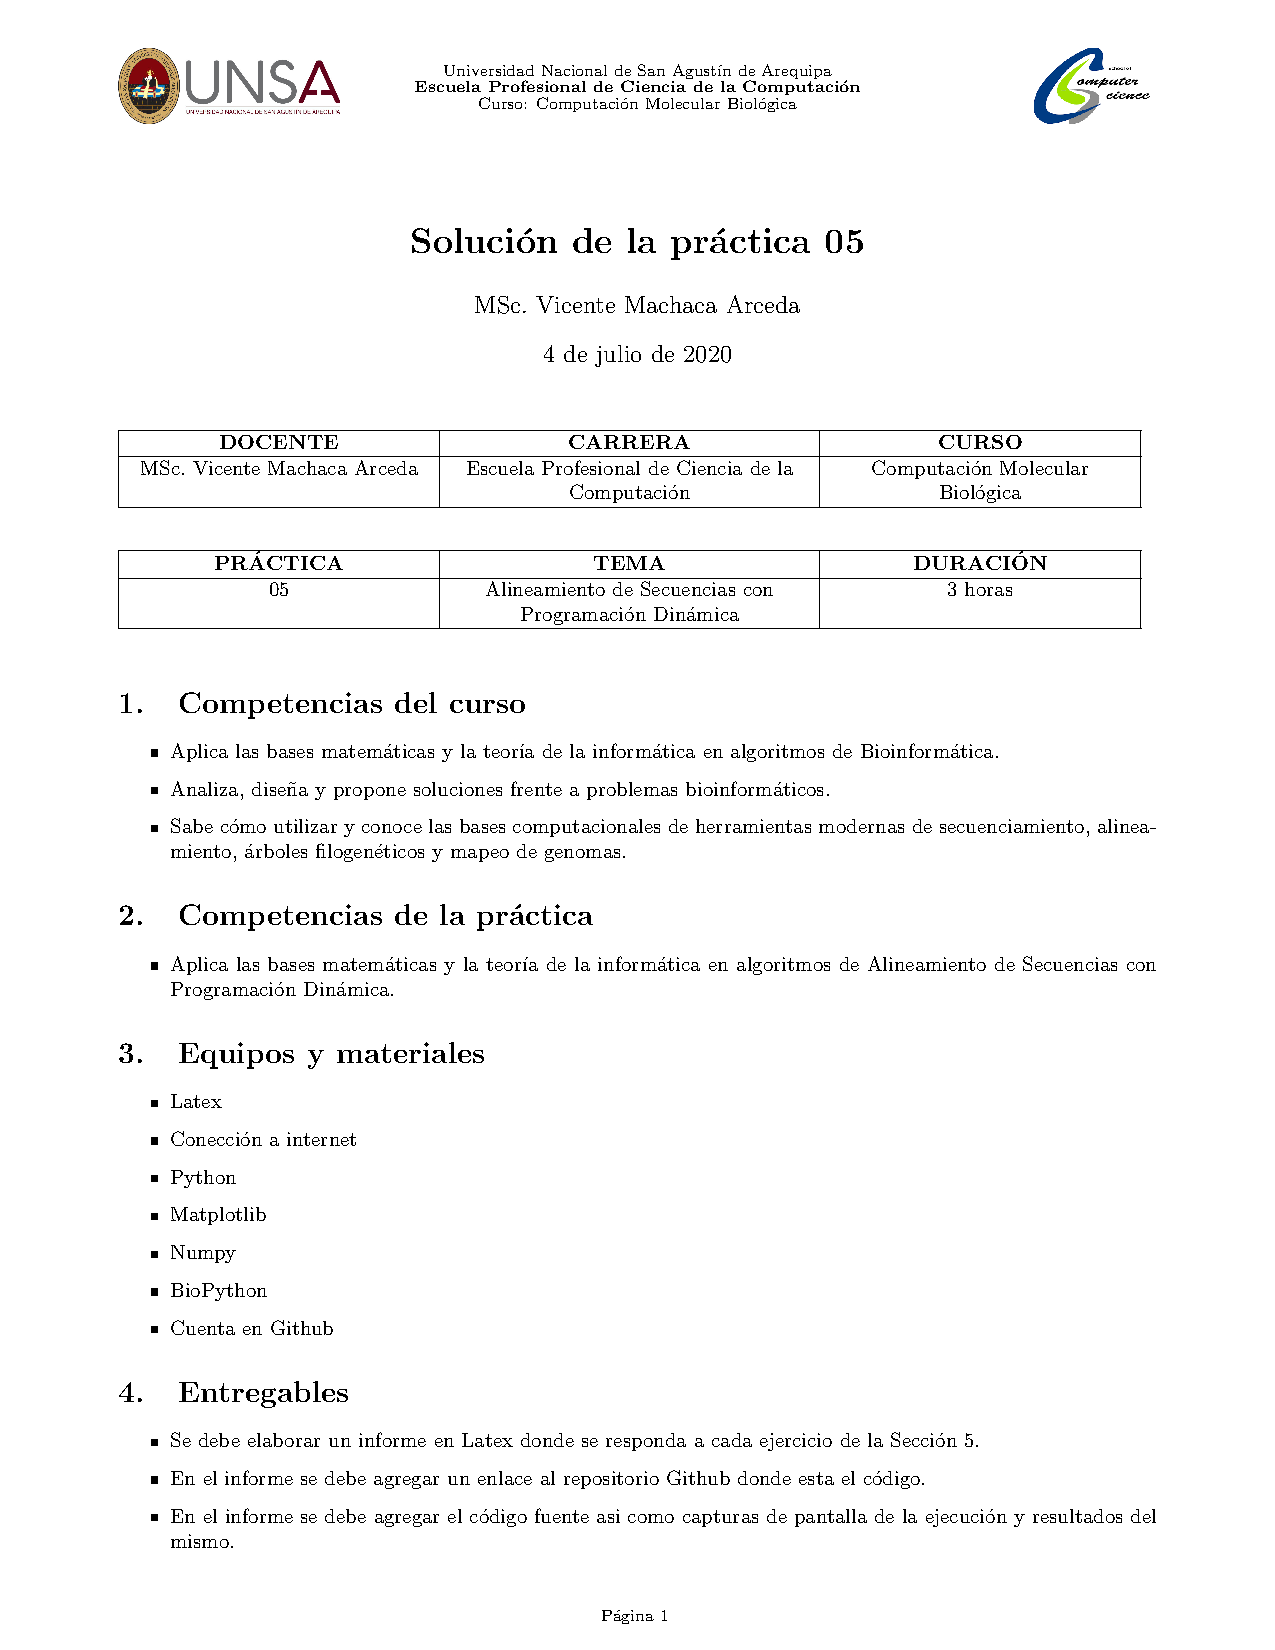
\includepdf[pages={1-}]{pdfs/practices/5_alignment_exercises_sol.pdf}

\pagestyle{empty} % Disable headers and footers for the following pages

\section{Evidencias}
La evidencia de los Laboratorios realizados por los estudiantes en la Evaluación Continua 2 se muestran en la siguiente tabla:

\begin{table}[h]
\centering
\begin{tabular}{l|c}
\hline
\textbf{Laboratorio} & 
\textbf{Evidencia} 
\\ \hline
Laboratorio 3 &
\href{https://drive.google.com/drive/folders/1knC3vddxB2suonXKBTW8DNcPRjSCXDQf?usp=sharing}{Link}
\\ \hline
Laboratorio 4 &
\href{https://drive.google.com/drive/folders/1Q-JOyVeBFSu1QmBeub5btlmi_CZmU5Wu?usp=sharing}{Link}
\\ \hline
Laboratorio 5  &
\href{https://drive.google.com/drive/folders/1q6vGtmIq2WdqRE3HXyVApg_rHB5SgpOs?usp=sharing}{Link}
\\ \hline
\end{tabular}
\caption{Evidencia Evaluación Continua 2}
\label{tab:evidencia_evaluacion_continua_2} % Unique label used for referencing the table in-text
%\addcontentsline{toc}{table}{Table \ref{tab:example}} % Uncomment to add the table to the table of contents
\end{table}
%------------------------------------------------

